%=======================02-713 LaTeX template, following the 15-210 template==================
%
% You don't need to use LaTeX or this template, but you must turn your homework in as
% a typeset PDF somehow.
%
% How to use:
%    1. Update your information in section "A" below
%    2. Write your answers in section "B" below. Precede answers for all 
%       parts of a question with the command "\question{n}{desc}" where n is
%       the question number and "desc" is a short, one-line description of 
%       the problem. There is no need to restate the problem.
%    3. If a question has multiple parts, precede the answer to part x with the
%       command "\part{x}".
%    4. If a problem asks you to design an algorithm, use the commands
%       \algorithm, \correctness, \runtime to precede your discussion of the 
%       description of the algorithm, its correctness, and its running time, respectively.
%    5. You can include graphics by using the command \includegraphics{FILENAME}
%
\documentclass[11pt]{article}
\usepackage{amsmath,amssymb,amsthm}
\usepackage{tikz}
\usetikzlibrary{arrows}
\usepackage{graphicx}
\usepackage[margin=1in]{geometry}
\usepackage{fancyhdr}
\usepackage{mathtools}
\usepackage{placeins}
\usepackage{listings}
\usepackage{color}

\definecolor{dkgreen}{rgb}{0,0.6,0}
\definecolor{gray}{rgb}{0.5,0.5,0.5}
\definecolor{mauve}{rgb}{0.58,0,0.82}

\lstset{frame=none,
  language=Java,
  aboveskip=3mm,
  belowskip=3mm,
  showstringspaces=false,
  columns=flexible,
  basicstyle={\small\ttfamily},
  numbers=none,
  numberstyle=\tiny\color{gray},
  keywordstyle=\color{blue},
  commentstyle=\color{dkgreen},
  stringstyle=\color{mauve},
  breaklines=true,
  breakatwhitespace=true,
  tabsize=3
}

\setlength{\parindent}{0pt}
\setlength{\parskip}{5pt plus 1pt}
\setlength{\headheight}{13.6pt}
\newcommand\question[2]{\vspace{.25in}\hrule\textbf{#1 #2}\vspace{.5em}\hrule\vspace{.10in}}
\renewcommand\part[1]{\vspace{.10in}\textbf{(#1)}}
\newcommand\algorithm{\vspace{.10in}\textbf{Algorithm: }}
\newcommand\correctness{\vspace{.10in}\textbf{Correctness: }}
\newcommand\runtime{\vspace{.10in}\textbf{Running time: }}
\pagestyle{fancyplain}
\lhead{\textbf{\NAME}}
\chead{\textbf{HW\HWNUM}}
\rhead{\today}
\begin{document}\raggedright
%Section A==============Change the values below to match your information==================
\newcommand\NAME{Sean Connor}  % your name
\newcommand\HWNUM{2}              % the homework number
%Section B==============Put your answers to the questions below here=======================

\question{Q1}{}
 \part{a}
\begin{lstlisting}
while( !main.isEmpty() ) // move all items to aux stack from main stack
	temp = main.pop()
	aux.push( temp )
i = temp // set i to temp, which is equal to the last (bottom) item of stack.
while( !aux.isEmpty() ) // move all items to main stack from aux stack
	main.push( aux.pop() )
\end{lstlisting}
\part{b}
\begin{lstlisting}
while( !mainstack.isEmpty() ) // move all items to aux stack from main stack
	aux.push( temp )
for ( a=0; a <= 2; a++ ) // move first three items to main stack from aux stack
	temp = aux.pop() // set temp variable to popped values
	main.push( temp )
i = temp // set i to temp, which is equal to the third item from bottom of stack
while( !aux.isEmpty() ) // move all remaining items to main stack from aux stack
	main.push( aux.pop() )
\end{lstlisting}

\newpage
\question{Q2}{} 
\part{a} 
\begin{table}[!htbp]
\centering
\begin{tabular}{lll}
Item & Description         & Stack  \\ \hline
\{   & push \{ onto stack  & \{     \\
{[}  & push {[} onto stack & \{{[}  \\
{]}  & pop {[} from stack  & \{     \\
{[}  & push {[} onto stack & \{{[}  \\
(    & push ( onto stack   & \{{[}( \\
)    & pop ( from stack    & \{{[}  \\
{]}  & pop {[} from stack  & \{    
\end{tabular}
\end{table}
Since there is still an item remaining in the stack at the end, the delimiters are not correct.

\part{b}
\begin{table}[!htbp]
\centering
\begin{tabular}{lll}
Item & Description         & Stack   \\ \hline
(    & push ( onto stack   & (       \\
(    & push ( onto stack   & ((      \\
)    & pop ( from stack    & (       \\
\{   & push \{ onto stack  & (\{     \\
(    & push ( onto stack   & (\{(    \\
{[}  & push {[} onto stack & (\{({[} \\
{]}  & pop {[} from stack  & (\{(    \\
)    & pop ( from stack    & (\{     \\
\}   & pop \{ from stack   & (       \\
)    & pop ( from stack    & empty  
\end{tabular}
\end{table}
Since the stack is empty, the delimiters are valid.
\FloatBarrier

\newpage
\question{Q3}{} 
\begin{lstlisting}
/* Java/pseudocode algorithm to check if str follows form x C y */
if( str=null OR str.length=0 OR charAt(0)=C OR charAt(str.length-1)=C ) // check if string is valid
	return false
else // string is valid, proceed
	i = 0
	while( charAt(i) != C ) // push all chars before C to aux stack
		aux.push( charAt(i) )
		i++
	temp = charAt(i) // set temp equal to C
	i++
	while( charAt(i) = aux.peek() ) // check if chars after C mimic/symmetric to chars before C
		aux.pop() // if so, pop from aux stack and check next char
		i++
		if( i = str.length) // break if end of string is reached
			break
	if( aux.isEmpty() ) // if stack is empty, string follows form
		return true
	else
		return false // if stack is not empty, string does not follow form
\end{lstlisting}

\newpage
\question{Q4}{} 
\begin{lstlisting}
/* Java/pseudocode algorithm to check if str follows form `a D b D c D ... D z' */
if( str=null OR str.length=0 OR charAt(0)=D OR charAt(str.length-1)=D ) // check if string is valid
	return false
else // string is valid, proceed
	start = 0
	for( int i = 0; i < str.length; i++ ) // iterate through every character in string
		if( charAt(i) = D ) 
			end = i
			valid = Problem3Solution( str.substring(start,end) ) // run the substring (string before/between/after D) through previous question solution
			if( valid = false ) // if Problem3Solution returns false, then this will return false to indicate string does not follow form
				return false
			start = end + 1 // set new substring start
	valid = Problem3Solution( str.substring(start,str.length) // run the last substring (following last D) through Problem3Solution method.
	if( valid = true )
		return true
	else
		return false
\end{lstlisting}

\newpage
\question{Q5}{} 
The requirement is to ``design and implement a stack in which each item on the stack is a varying number of integers." I interpret this to mean that each item in the stack is an array of integers. Thus, the stack can be implemented by the int[][] data type, also known as a 2D int array or an array of int arrays. In Java, the size of the arrays must be declared upon creation (or specify the array literals); however, each element in the `primary' array can be explicitly set to a different size after initialization.
\begin{lstlisting}
/* Java/pseudocode to implement stack with int[] elements */
size = 10 // set static stack size
top = -1 // set top of empty stack to -1 (since first element will be at index 0)
int[][] stack = new int[size][1]; // creates a stack of size ten, initialized with ten int[1] arrays (which initialize to zero by default)

/* push method */
if( top < size-1 )
	top++
	stack[top] = element // element is an int[]
else
	no room to add!

/* pop method */
if( top > -1 )
	temp = stack[top]
	top--
	return temp
else
	nothing to pop!

/* empty method */
if( top == -1 )
	return true
else
	return false
\end{lstlisting}

\newpage
\question{Q6}{} 
There are four primary functions for the 1D array - insert to end, delete from end, insert at i\textsuperscript{th} element, and delete  i\textsuperscript{th} element. The main stack is representative of the array, and the auxiliary stack is used for insert and delete functions. 
\begin{itemize}
	\item insert to end $\rightarrow$ push to main stack
	\item delete from end $\rightarrow$ pop from main stack
	\item insert at i\textsuperscript{th} $\rightarrow$
		\begin{enumerate}
			\item move all items to aux stack
			\item move i-1 items back to main stack
			\item push insert item to main stack
			\item move remainder of items back to main stack
		\end{enumerate}
	\item delete  i\textsuperscript{th}  $\rightarrow$
		\begin{enumerate}
			\item move all items to aux stack
			\item move i-1 items back to main stack
			\item pop  i\textsuperscript{th} item
			\item move remainder of items back to main stack
		\end{enumerate}
\end{itemize}

\newpage
\question{Q7}{}
This can be accomplished by having one stack start at 0 and increase in size (top of stack i++). The other stack would start at array.length-1 and increase in size by moving the top of the stack towards 0 (top of stack i--).
\begin{figure}[!h]
\centering
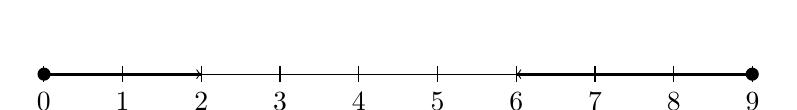
\begin{tikzpicture} 
\draw (0,0) -- (9,0) ; %edit here for the axis
\foreach \x in  {0,1,2,3,4,5,6,7,8,9} % edit here for the vertical lines
\draw[shift={(\x,0)},color=black] (0pt,3pt) -- (0pt,-3pt);
\foreach \x in {0,1,2,3,4,5,6,7,8,9} % edit here for the numbers
\draw[shift={(\x,0)},color=black] (0pt,0pt) -- (0pt,-3pt) node[below] 
{$\x$};
\draw[*->] (-.08,0) -- (2,0);
\draw[very thick] (0,0) -- (2,0);
\draw[<-*] (6,0) -- (9.08,0);
\draw[very thick] (6,0) -- (9,0);
\end{tikzpicture}
\end{figure}
\begin{lstlisting}
/* Java/pseudocode to implement two stacks in single array */
s = new int[size]
top1 = -1
top2 = size

/* push1 method Java/pseudocode */
if( top1 < top2-1 ) 
	top1++
	s[top1] = item
else
	no room to push!

/* pop1 method Java/pseudocode */
if( top1 >= 0 )
	item = s[top1]
	top1--
	return item
else 
	nothing to pop!

/* push2 method Java/pseudocode */
if( top1 < top2-1 )
	top2--
	s[top2] = item
else 
	no room to push!

/* pop2 method Java/pseudocode */
if( top2 < size )
	item = s[top2]
	top2++
	return item
else
	nothing to pop!
\end{lstlisting}

\newpage
\question{Q8}{} 
\part{a}
Prefix
\begin{gather*}
(A+B)*(C\$(D-E)+F)-G \\
(+AB)*(C\$(-DE)+F)-G \\
(+AB)*(\$C-DE)+F)-G \\
(+AB)*(+\$C-DEF)-G \\
\fbox{-*+AB+\$C-DEFG}
\end{gather*}
Postfix
\begin{gather*}
(A+B)*(C\$(D-E)+F)-G \\
(AB+)*(C\$(DE-)+F)-G \\
(AB+)*(CDE-\$)+F)-G \\
(AB+)*(CDE-\$F+)-G \\
(AB+CDE-\$F+*)-G \\
\fbox{AB+CDE-\$F+*G-}
\end{gather*}
\part{b}
Prefix
\begin{gather*}
A+(((B-C)*(D-E)+F)/G)\$(H-J) \\
A+(((-BC)*(-DE)+F/G)(-HJ) \\
A+\$((*(-BC-DE)+F)/G)(-HJ) \\
A+\$((+*-BC-DEF)/G)(-HJ) \\
A+\$/+*-BC-DEFG-HJ \\
\fbox{+A\$/+*-BC-DEFG-HJ}
\end{gather*}
Postfix
\begin{gather*}
A+(((B-C)*(D-E)+F)/G)\$(H-J) \\
A+(((BC-DE-*)+F)/G)\$(HJ-) \\
A+((BC-DE-*F+)/G)\$(HJ-) \\ 
A+(BC-DE-*F+G/)\$(HJ-) \\
A+(BC-DE-*F+G/HJ-\$) \\
\fbox{ABC-DE-*F+G/HJ-\$+)}
\end{gather*}

\newpage
\question{Q9}{} 
\part{a}
\begin{table}[!htbp]
\centering
\begin{tabular}{ll}
Item & Stack              \\ \hline
I    & I                  \\
H    & I,H                \\
G    & I,H,G              \\
*    & I,G*H              \\
F    & I,G*H,F            \\
E    & I,G*H,F,E          \\
+    & I,G*H,E+F          \\
/    & I,E+F/G*H          \\
D    & I,E+F/G*H,D        \\
C    & I,E+F/G*H,D,C      \\
B    & I,E+F/G*H,D,C,B    \\
\$   & I,E+F/G*H,D,B\$C   \\
*    & I,E+F/G*H,B\$C*D   \\
-    & I,B\$C*D-E+F/G*H   \\
A    & I,B\$C*D-E+F/G*H,A \\
+    & I,A+B\$C*D-E+F/G*H \\
+    & \fbox{A+B\$C*D-E+F/G*H+I}
\end{tabular}
\end{table}
\FloatBarrier
\part{b}
\begin{table}[!htbp]
\centering
\begin{tabular}{ll}
Item & Stack          \\ \hline
G    & G              \\
F    & G,F            \\
E    & G,F,E          \\
*    & G,E*F          \\
*    & E*F*G          \\
D    & E*F*G,D        \\
*    & D*E*F*G        \\
C    & D*E*F*G,C      \\
B    & D*E*F*G,C,B    \\
A    & D*E*F*G,C,B,A  \\
\$   & D*E*F*G,C,A\$B \\
-    & D*E*F*G,A\$B-C \\
+    & \fbox{A\$B-C+D*E*F*G}
\end{tabular}
\end{table}
\FloatBarrier
\newpage
\part{c}
\begin{table}[!htbp]
\centering
\begin{tabular}{ll}
Item & Stack        \\ \hline
A    & A            \\
B    & A,B          \\
-    & A-B          \\
C    & A-B,C        \\
+    & A-B+C        \\
D    & A-B+C,D      \\
E    & A-B+C,D,E    \\
F    & A-B+C,D,E,F  \\
-    & A-B+C,D,E-F  \\
+    & A-B+C,D+E-F  \\
\$   & \fbox{A-B+C\$D+E-F}
\end{tabular}
\end{table}
\FloatBarrier
\part{d}
\begin{table}[!htbp]
\centering
\begin{tabular}{ll}
Item & Stack          \\ \hline
A    & A              \\
B    & A,B            \\
C    & A,B,C          \\
D    & A,B,C,D        \\
E    & A,B,C,D,E      \\
-    & A,B,C,D-E      \\
+    & A,B,C+D-E      \\
\$   & A,B\$C+D-E     \\
*    & A*B\$C+D-E     \\
E    & A*B\$C+D-E,E   \\
F    & A*B\$C+D-E,E,F \\
*    & A*B\$C+D-E,E*F \\
-    & \fbox{A*B\$C+D-E-E*F}
\end{tabular}
\end{table}
\FloatBarrier

\newpage
\question{Q10}{} 
\part{a}
\begin{gather*}
AB+C-BA+C\$- \quad A=1; \; B=2; \; C=3\\
(1+2)-3-(2+1)^3 \\
3 - 3 - 3^3 \\
0 - 3^3 \\
0 - 27 \\
\fbox{-27}
\end{gather*}
\part{b}
\begin{gather*}
ABC+*CBA-+*  \quad A=1; \; B=2; \; C=3\\
1*(2+3)*(3+(2-1)) \\
(1*5) * (3+1) \\
5*4 \\
\fbox{20}
\end{gather*}

\newpage
\question{Q11}{}
The general algorithm is the following:
\begin{itemize}
	\item add string to main stack, left to right
	\item run the following until main stack is empty
	\begin{itemize}
		\item if top of main stack is operand, add to final stack
		\item if top of main stack is `)' or operator with equal or higher precedence than top of opstack, add to opstack
		\item if top of main stack is `(', pop `(' from main stack, move operators from opstack to final stack until `)' is encountered, then pop the `)' from opstack
		\item if top of main stack is operator with lower precedence than top of opstack, pop opstack to final stack until top of main stack is no longer lower precedence, then pop top of main stack to opstack.
	\end{itemize}
	\item finally, move remainder of opstack to final stack
	\item convert final stack back to string in regular order to obtain prefix expression string	
\end{itemize}
\begin{lstlisting}
/* Java/pseudocode for conversion of infix string to prefix string */
for( i=0; i< str.length; i++) // move all chars in string to main stack
	main.push( charAt(i) )

while( !main.isEmpty ) // run until main stack is empty
	if( main.peek is operand) // if top of main stack is operand, move to final stack
		final.push( main.pop() )
	
	elseif( main.peek = ')' OR operatorHierarchy( main.peek ) >= operatorHierarchy( opstack.top ) ) // if top of main stack is ')' or has higher priority than top of opstack, add to opstack
		opstack.push( main.pop() )
	
	elseif( main.peek = '(' ) // if top of main stack is '(' then add all from opstack to final stack until reaching a ')' in opstack
		main.pop()
		while( opstack.peek != ')' )
			final.push( opstack.pop() )
		opstack.pop() // pop ')' from opstack
	
	elseif(  operatorHierarchy( main.peek ) < operatorHierarchy( opstack.top ) ) //  if top of main stack is has lower priority than top of opstack, add top of opstack to final stack and top of main stack to opstack
		while( !opstack.isEmpty AND (operatorHierarchy( main.peek ) < operatorHierarchy( opstack.top )) )
			final.push( opstack.pop() )
			opstack.push( main.pop() )

while( !opstack.isEmpty ) // main stack is empty, add what's left of opstack to final stack
	final.push( opstack.pop() )
\end{lstlisting}

\newpage
\question{Q12}{} 
The answer is lg(n) rounded up to the nearest whole number. This is given by:
\begin{gather*}
\frac{n}{2^{max}} < 1
\end{gather*}
For example, in the following figure if our search is for 0, we could halve (round up) and guess element 5. 0 is less than five so it must be between elements 0 and 4. We could halve again and guess element 2. We could halve again and guess element 1. Finally, the only remaining item is element 0. Thus, depending on how the search is executed, one could say it took at most three calls (lg(n) rounded down to nearest whole) if you go by process of elimination, or four calls (lg(n) rounded up to nearest whole) if you actually use the search algorithm to 'land' on the desired value.
\begin{figure}[!h]
\centering
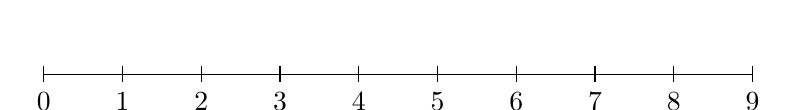
\begin{tikzpicture} 
\draw (0,0) -- (9,0) ; %edit here for the axis
\foreach \x in  {0,1,2,3,4,5,6,7,8,9} % edit here for the vertical lines
\draw[shift={(\x,0)},color=black] (0pt,3pt) -- (0pt,-3pt);
\foreach \x in {0,1,2,3,4,5,6,7,8,9} % edit here for the numbers
\draw[shift={(\x,0)},color=black] (0pt,0pt) -- (0pt,-3pt) node[below] 
{$\x$};
\end{tikzpicture}
\end{figure}

\newpage
\question{Q13}{}
Three cases are provided. One of them serves as a base case that returns an integer. The other two are already described as calling the gcd method again. Thus, the recursive method is as follows:
\begin{lstlisting}
/* Java/pseudocode for recursive GCD method */
GCD(int x, int y){
if( y <= x AND x%y == 0 )
	return y	
else if( x < y )
	return GCD(y,x)
else
	return GCD(y,x%y)
}
\end{lstlisting}

\end{document}









